\section{Result Analysis}
\label{ch:results}
\subsection{Test sample and reporting conventions}
The primary test comprises 334 daily predictions, with last input days from 1 October 2025 to 30 August 2026. Of these days, 162 were followed by a rise and 172 were not, giving an up-share of 48.50\%. Every headline comparison uses the same days and outcomes.

Two kinds of figure are reported. The \emph{mean} is the average of a metric over ten separately trained seeds. The \emph{ensemble} value is computed after averaging the ten models' probabilities for each day. The two need not coincide. If individual models fall on opposite sides of 0.5, their average can fall on either side, so ensemble accuracy is not the mean of the seed accuracies. The majority rule is run once and has no seed spread.

\subsection{Main next-day results}
\begin{table}[htbp]\centering\small
\caption{Primary held-out results on the 334 common test days. Mean $\pm$ SD is across seeds; ensemble columns use averaged probabilities.}\label{tab:mainresults}
\begin{tabularx}{\textwidth}{Xrrrr}
\toprule
Model & Mean acc. (\%) & SD (pp) & Ensemble acc. (\%) & Ensemble bal. acc. (\%)\\\midrule
Training-majority rule & 51.50 & --- & 51.50 & 50.00\\
LSTM A, price only & 48.71 & 1.41 & 50.00 & 49.82\\
LSTM B, price + VADER & 47.84 & 0.97 & 48.50 & 48.30\\
XGBoost, price only & 47.69 & 2.26 & 49.40 & 49.24\\
XGBoost, price + VADER (extra) & 48.68 & 2.43 & 47.90 & 47.71\\
LSTM B, price + FinBERT (secondary) & 48.53 & 1.24 & 47.90 & 47.70\\
\bottomrule
\end{tabularx}
\end{table}

The answer to RQ1 is negative. Model A reached 50.00\% and Model B with VADER 48.50\%, whereas the majority rule, which makes no attempt to read the market, scored 51.50\%. This does not indicate that the networks failed to train, since they learned structure from the training years. That structure did not translate into more correct calls on the held-out days.

\figurewide{accuracy_comparison.pdf}{Ensemble test accuracy of the main and secondary models. The dashed line is 50\%, although the actual majority baseline reaches 51.50\%.}{fig:comparison}

Precision, recall and F1 complete the picture. The majority rule never predicts a rise, so its positive-class precision, recall and F1 are zero by the convention of the evaluation code. It nevertheless leads on accuracy because the test period contains slightly more not-up days. The LSTMs predict both classes, but the additional rises they identify are offset by false alarms.

\begin{table}[htbp]\centering\small
\caption{Positive-class metrics of the ensembles on the main test split}\label{tab:prf}
\begin{tabularx}{\textwidth}{Xrrrr}
\toprule
Model & Precision (\%) & Recall (\%) & F1 (\%) & Balanced acc. (\%)\\\midrule
Majority not-up & 0.00 & 0.00 & 0.00 & 50.00\\
LSTM A & 48.30 & 43.83 & 45.95 & 49.82\\
LSTM B / VADER & 46.53 & 41.36 & 43.79 & 48.30\\
XGBoost / price & 47.65 & 43.83 & 45.66 & 49.24\\
LSTM B / FinBERT & 45.83 & 40.74 & 43.14 & 47.70\\
\bottomrule
\end{tabularx}
\end{table}

\subsection{Predictions against outcomes over time}
A single accuracy figure conceals how a model behaves from week to week. Figure~\ref{fig:predicted} therefore follows the test period day by day. Panel (a) shows the actual price, with the calls of the price-only LSTM marked as right or wrong. The model was right on 167 days and wrong on 167. The wrong calls are scattered along the whole path, and nothing in the figure suggests that the model reads the trend.

Panel (b) compares predicted probabilities with the outcomes. The black line is the share of up days in the preceding seven. It varies between 0 and 1, because seven-day stretches in this period were sometimes entirely up or entirely down. The blue and orange lines are the seven-day averages of the predicted probability of a rise for Models A and B. They remain close to 0.5. For Model A the seven-day average lies between 0.45 and 0.66, and for Model B between 0.44 and 0.62, while single-day probabilities for Model A range from 0.42 to 0.75. The networks therefore do not follow the swings in the ground truth. It appears that they learned to stay near 50\%, which is what a model does when the features carry little signal and the loss rewards caution.

Panel (c) shows rolling 30-day accuracy. Model A moves between 36.7\% and 70.0\%, Model B (VADER) between 33.3\% and 63.3\%, and the majority rule between 33.3\% and 73.3\%. No model remains ahead of the others for long, and the lead changes every few weeks. This is consistent with a result that is close to chance and is shaped by whichever month happens to suit a particular model.

\begin{figure}[htbp]\centering
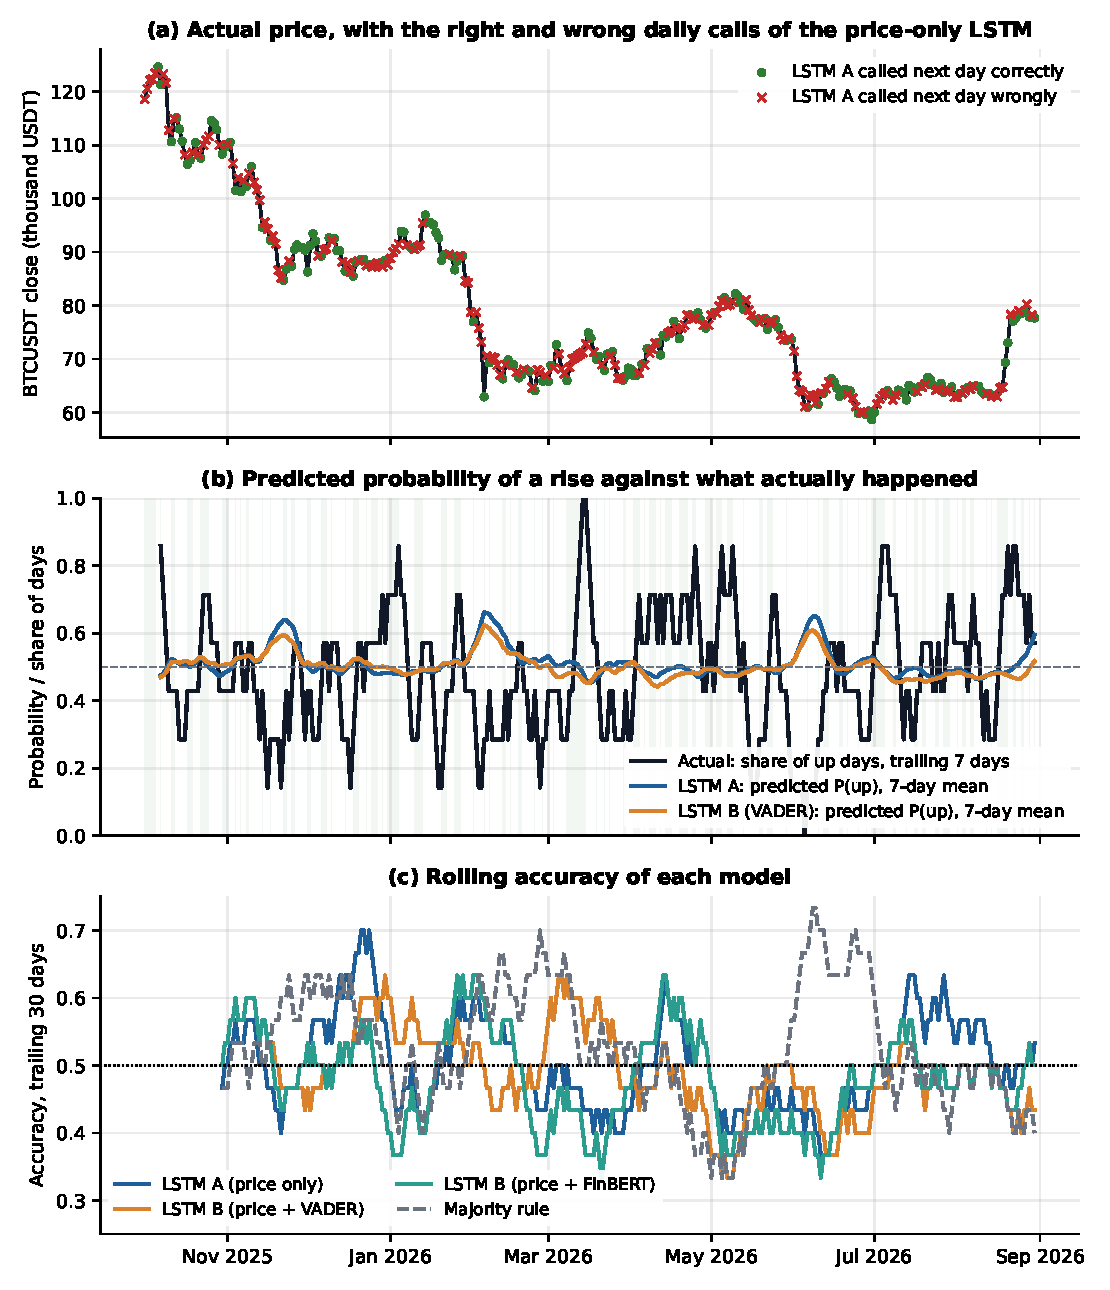
\includegraphics[width=0.93\textwidth]{figures/predicted_vs_actual.pdf}
\caption{Predictions against outcomes on the 334 test days. (a) Actual close, with right and wrong calls of LSTM A. (b) Trailing 7-day share of up days against the 7-day average predicted probability of a rise. (c) Trailing 30-day accuracy of each model.}\label{fig:predicted}
\end{figure}

\subsection{Confusion matrices}
The confusion matrix shows what the accuracy figure compresses. For the price-only LSTM, 96 not-up days and 71 up days were called correctly. A further 76 not-up days were wrongly called up, and 91 up days were missed. That gives 167 correct calls out of 334. The VADER model has 95 true negatives and 67 true positives, a total of 162 correct calls, five fewer than Model A.

\begin{table}[htbp]\centering
\caption{Ensemble confusion counts (rows give the actual outcome)}\label{tab:confusion}
\begin{tabular}{lrrrr}
\toprule
Model & TN & FP & FN & TP\\\midrule
Majority rule & 172 & 0 & 162 & 0\\
LSTM A & 96 & 76 & 91 & 71\\
LSTM B / VADER & 95 & 77 & 95 & 67\\
XGBoost price & 94 & 78 & 91 & 71\\
LSTM B / FinBERT & 94 & 78 & 96 & 66\\
\bottomrule
\end{tabular}
\end{table}

\figurewide{confusion_matrices.pdf}{Confusion matrices of the majority baseline and the two primary LSTM ensembles. Rows are the actual class and columns the predicted class.}{fig:cms}

Every model that predicts both directions faces the same trade-off. The additional correct rises must outweigh the additional false alarms on flat or falling days, and here they do not. Balanced accuracy remains close to 50\%, so the networks behave as weak classifiers.

\subsection{The sentiment effect and its uncertainty}
The primary sentiment effect is the difference between the matched ensembles,
\[
\Delta_{B-A}=0.48503-0.50000=-0.01497,
\]
or $-1.50$ percentage points. Balanced accuracy falls by 1.53 points. The paired bootstrap resamples the 334 days 2,000 times, always drawing the outcomes of Models A and B for the same days.

\begin{table}[htbp]\centering\small
\caption{Paired ensemble comparisons (Model B minus Model A)}\label{tab:delta}
\begin{tabularx}{\textwidth}{Xrrr}
\toprule
Difference & Point (pp) & 95\% interval (pp) & Excludes zero?\\\midrule
VADER B -- A, accuracy & $-1.50$ & $[-5.69,\ +2.40]$ & No\\
VADER B -- A, balanced accuracy & $-1.53$ & $[-5.71,\ +2.51]$ & No\\
FinBERT B -- A, accuracy & $-2.10$ & $[-5.40,\ +1.20]$ & No\\
FinBERT B -- VADER B, accuracy & $-0.60$ & $[-4.19,\ +3.00]$ & No\\
\bottomrule
\end{tabularx}
\end{table}

All four intervals include zero. The point estimates favour the simpler model, but the data cannot establish that sentiment is harmful, since a small gain and a moderate loss are both compatible with the intervals. The supportable conclusion is narrower: neither sentiment source showed a dependable benefit.

\subsection{From validation to test}
Model A's ensemble scored 57.14\% on validation and 50.00\% on test, a decrease of 7.14 points. Model B (VADER) fell from 52.75\% to 48.50\%, or 4.25 points, and XGBoost also lost ground. The models therefore learned relationships that did not carry fully into the later period, although a single split cannot indicate whether the cause was a changing market, selection optimism or both.

\figurewide{validation_vs_test.pdf}{Ensemble accuracy on validation and test days, from the saved evaluation files.}{fig:valtest}

Validation figures are flattered for a simple reason. The validation days helped to select the settings and the stopping epochs, so some optimism is built in even though the test days were never consulted. The 17-day news gap also lies in the validation period and not in the test period, which makes the two feature distributions differ.

\subsection{Probabilities clustered near the threshold}
With 334 days, the 95\% half-width for a guessing model is about 5.4 percentage points under independence. Serial dependence probably makes that figure optimistic. In either case, differences of one or two points are not persuasive.

The stored probabilities add a further observation. About 81.4\% of Model A's test predictions and 82.6\% of Model B's lie between 0.45 and 0.55. The networks are rarely confident, so a small change in a probability can alter a call. This describes the saved predictions and is not a new experiment.

\figurewide{probability_histograms.pdf}{Distribution of ensemble probabilities on the test days. Most lie close to the 0.5 threshold.}{fig:histprob}

\subsection{Walk-forward evaluation}
A single test window can flatter or penalise a model by chance, so the comparison was repeated eight times. Each period of about six months was tested by models retrained on all earlier data, using the same frozen settings and ten seeds. Together the periods cover 1,338 days from January 2023 to August 2026.

\begin{table}[htbp]\centering\small
\caption{Walk-forward results pooled over 1,338 test days. The guessing band is $50\% \pm 2.7$ points.}\label{tab:wfpooled}
\begin{tabularx}{\textwidth}{Xrrrr}
\toprule
Model & Mean acc. (\%) & SD (pp) & Ensemble acc. (\%) & Ensemble bal. acc. (\%)\\\midrule
Majority rule & 49.40 & --- & 49.40 & 50.00\\
XGBoost, price only & 48.86 & 0.48 & 47.53 & 47.75\\
LSTM A, price only & 51.19 & 0.96 & 51.42 & 51.60\\
LSTM B, price + VADER & 50.35 & 0.87 & 50.00 & 50.03\\
LSTM B, price + FinBERT & 50.89 & 0.70 & 52.17 & 52.26\\
\bottomrule
\end{tabularx}
\end{table}

The pooled picture agrees with the single split. Every model lies within about two points of 50\%, and the highest ensemble figure, 52.17\% for FinBERT, is still inside the guessing band. The sentiment effect also remains within the noise. VADER Model B minus Model A is $-1.42$ points (95\% interval $-4.04$ to $+1.05$), and FinBERT Model B minus Model A is $+0.75$ points ($-1.64$ to $+3.07$), using blocks of seven days to allow for correlated errors. Model B exceeded Model A in three of eight periods with VADER and in four of eight with FinBERT, which is about what chance would produce.

Table~\ref{tab:wffolds} shows how strongly the results vary between periods.

\begin{table}[htbp]\centering\small
\caption{Ensemble accuracy (\%) in each walk-forward period}\label{tab:wffolds}
\begin{tabularx}{\textwidth}{lrrrrrrr}
\toprule
Test period & Days & Up (\%) & Majority & XGBoost & LSTM A & B (VADER) & B (FinBERT)\\\midrule
Jan--Jun 2023 & 181 & 50.3 & 49.7 & 50.8 & 50.8 & 49.2 & 50.8\\
Jul--Dec 2023 & 184 & 50.5 & 49.5 & 46.7 & 49.5 & 53.3 & 55.4\\
Jan--Jun 2024 & 182 & 52.8 & 47.3 & 47.3 & 53.3 & 55.5 & 54.4\\
Jul--Dec 2024 & 184 & 52.2 & 47.8 & 47.8 & 53.3 & 47.8 & 52.2\\
Jan--Jun 2025 & 181 & 50.8 & 49.2 & 51.9 & 55.2 & 55.2 & 58.0\\
Jul--Dec 2025 & 184 & 49.5 & 50.5 & 47.8 & 53.3 & 47.8 & 50.0\\
Jan--Jun 2026 & 181 & 45.9 & 54.1 & 39.8 & 47.5 & 42.0 & 44.2\\
Jul--Aug 2026 & 61 & 57.4 & 42.6 & 49.2 & 42.6 & 47.5 & 52.5\\
\bottomrule
\end{tabularx}
\end{table}

Accuracy ranges from 39.8\% to 58.0\% across the cells, and it appears to follow the market's mix of up and down days more than it follows the model. January to June 2026 is the weakest full six-month period for every learned model, and only 45.9\% of its days closed higher. The majority rule, which predicts ``not up'' on every day, wins that period with 54.1\%. This is what pulled the main test result below 50\%, since the test window overlaps the last three periods. The strongest stretch, the first half of 2025, lies inside the validation window used to choose settings and is probably flattered. The two effects cannot be separated with these data.

\begin{figure}[htbp]\centering
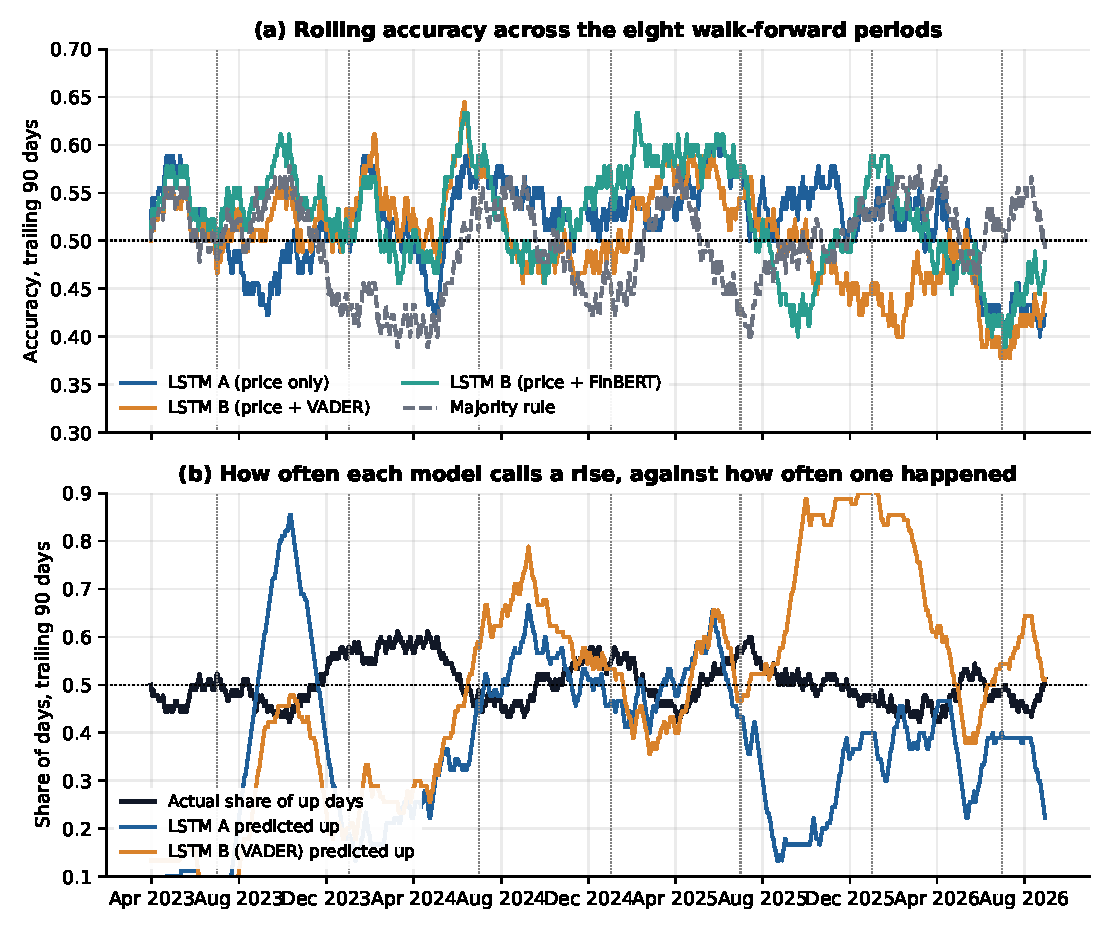
\includegraphics[width=0.93\textwidth]{figures/walkforward_rolling.pdf}
\caption{Walk-forward predictions over time, 2023 to 2026. (a) Rolling 90-day accuracy. (b) Share of days each model called a rise, against the share of days that actually rose. Dotted lines mark the start of each period.}\label{fig:wfroll}
\end{figure}

Figure~\ref{fig:wfroll} presents the curves over the full span. Rolling 90-day accuracy for LSTM A ranges from 40.0\% to 61.1\%, for B (VADER) from 37.8\% to 64.4\% and for B (FinBERT) from 38.9\% to 63.3\%. Panel (b) is more informative. The actual share of up days barely changes, from 42.2\% to 61.1\% in any 90-day window, whereas the models' share of rise calls ranges from 2.2\% to 85.6\% for Model A and from 3.3\% to 92.2\% for Model B. The models alternate between predicting almost every day up and almost every day down for months at a time, without tracking the real mix.

\figurewide{walkforward_folds.pdf}{Ensemble accuracy of each model in the eight walk-forward periods. The dotted line is 50\%.}{fig:wffolds}

\subsection{Does sentiment lead or follow price?}
The preceding results indicate that sentiment does not help. The lag analysis examines why. For each day it correlates the sentiment on day $t$ with the return on day $t+k$, for $k$ from $-5$ to $+5$. The sample is the 1,617 days from January 2021 to mid-June 2025, and the measure is Spearman's rank correlation \cite{spearman1904}.

\begin{figure}[htbp]\centering
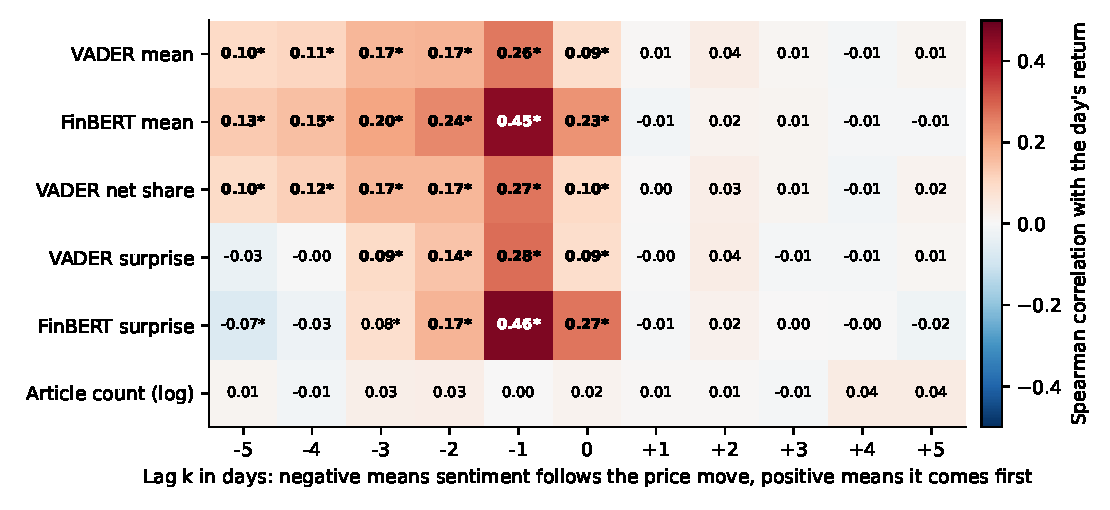
\includegraphics[width=0.95\textwidth]{figures/lag_heatmap.pdf}
\caption{Spearman correlation between day-$t$ sentiment and the return on day $t+k$. An asterisk marks a nominal $p<0.05$, and bold type marks significance after correction for 132 tests.}\label{fig:lag}
\end{figure}

The pattern in Figure~\ref{fig:lag} is asymmetric. Sentiment is associated with moves that have already happened. FinBERT's daily mean correlates 0.449 with the previous day's return ($k=-1$) and 0.225 with the same day's, whereas VADER's mean gives 0.262 and 0.089. Looking forward, the association disappears. At $k=+1$, the day the models predict, the correlations are $-0.012$ for FinBERT and $+0.005$ for VADER, with permutation $p$-values of 0.60 and 0.84.

Of the 132 tests, 32 reached $p<0.05$ against about 7 expected by chance, and 25 remained significant after a Bonferroni correction for the number of tests \cite{dunn1961}. All 25 have $k\leq0$. None of the tests with $k\geq1$ reached even $p<0.05$. Headlines on a given UTC day thus mostly describe the preceding day, so that by the time a score exists the price has already responded. The article count was likewise uninformative about the size of the next move.

Grouping days by sentiment level leads to the same conclusion. Across the five VADER groups the share of days followed by a rise ranges from 48.8\% to 51.7\%, and across the FinBERT groups from 47.7\% to 53.1\%, with no steady trend from pessimistic to optimistic days. The same-day association also varies from year to year (0.11 to 0.32 for FinBERT, $-0.02$ to $+0.12$ for VADER), which makes it a weak basis for a predictive model.

All 18 model inputs were also screened against the next day's direction. Five reached $p<0.05$ against 0.9 expected by chance, and three remained significant after correction: the daily return, the log return and the ratio of the close to its 7-day average. All three have negative sign. After an up day the next day is slightly more likely to be down, with an area under the ROC curve of about 0.55 once the sign is reversed \cite{fawcett2006}. No sentiment input came close. The reversal did not carry into the test period either, where every model remained near 48\%, so it should not be regarded as a stable signal.

\subsection{Monthly behaviour}
Month by month, Model A's test accuracy ranges from 45.2\% to 54.8\% and Model B's from 40.0\% to 61.3\%. With only 28 to 31 days per month, each figure carries a wide margin of error, and the plot is best read as a reminder that 50\% is an average of very uneven months.

\figurewide{monthly_test_accuracy.pdf}{Monthly test accuracy of the two LSTM ensembles. Each month has 28 to 31 days, so single-month differences carry little weight.}{fig:monthly}

\subsection{Summary}
Four findings stand out. The LSTMs do not beat the majority rule on the frozen test days. Adding sentiment from either VADER or FinBERT gives no dependable gain, on one split or across eight. The predicted probabilities remain near 50\%, and the calls drift between near-constant up and near-constant down over time. And sentiment correlates with past returns far more than with future ones, which offers a direct explanation of why it fails to forecast the next day.
